% Editable native annotations around unchanged verified IDE photographs.
\par
\begin{figure}[htbp]
  \centering
  \sbox0{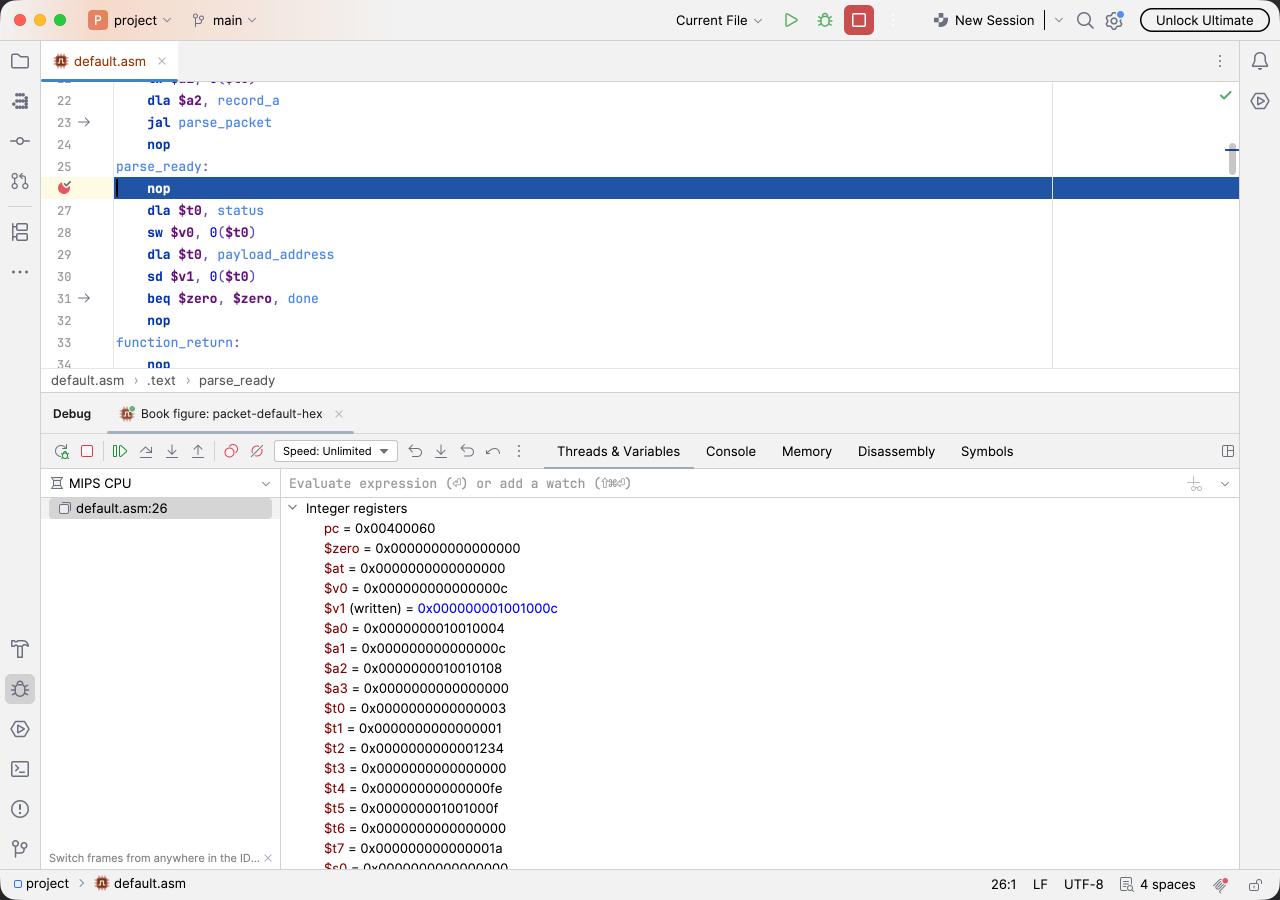
\includegraphics[artifact]{packages/013-binary-packet-parser/captures/f01-default/hex.png}}
  \sbox2{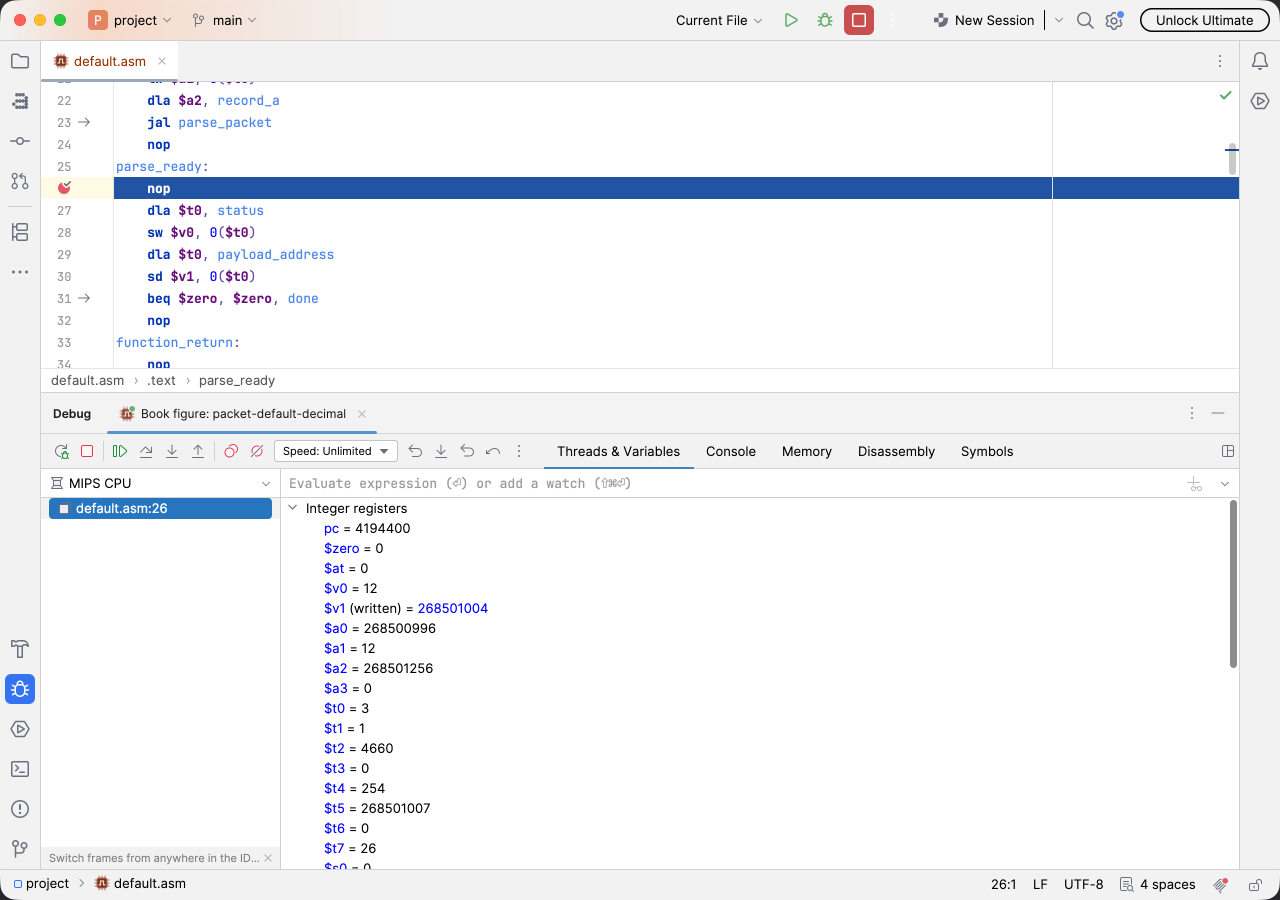
\includegraphics[artifact]{packages/013-binary-packet-parser/captures/f01-default/decimal.png}}
  \sbox4{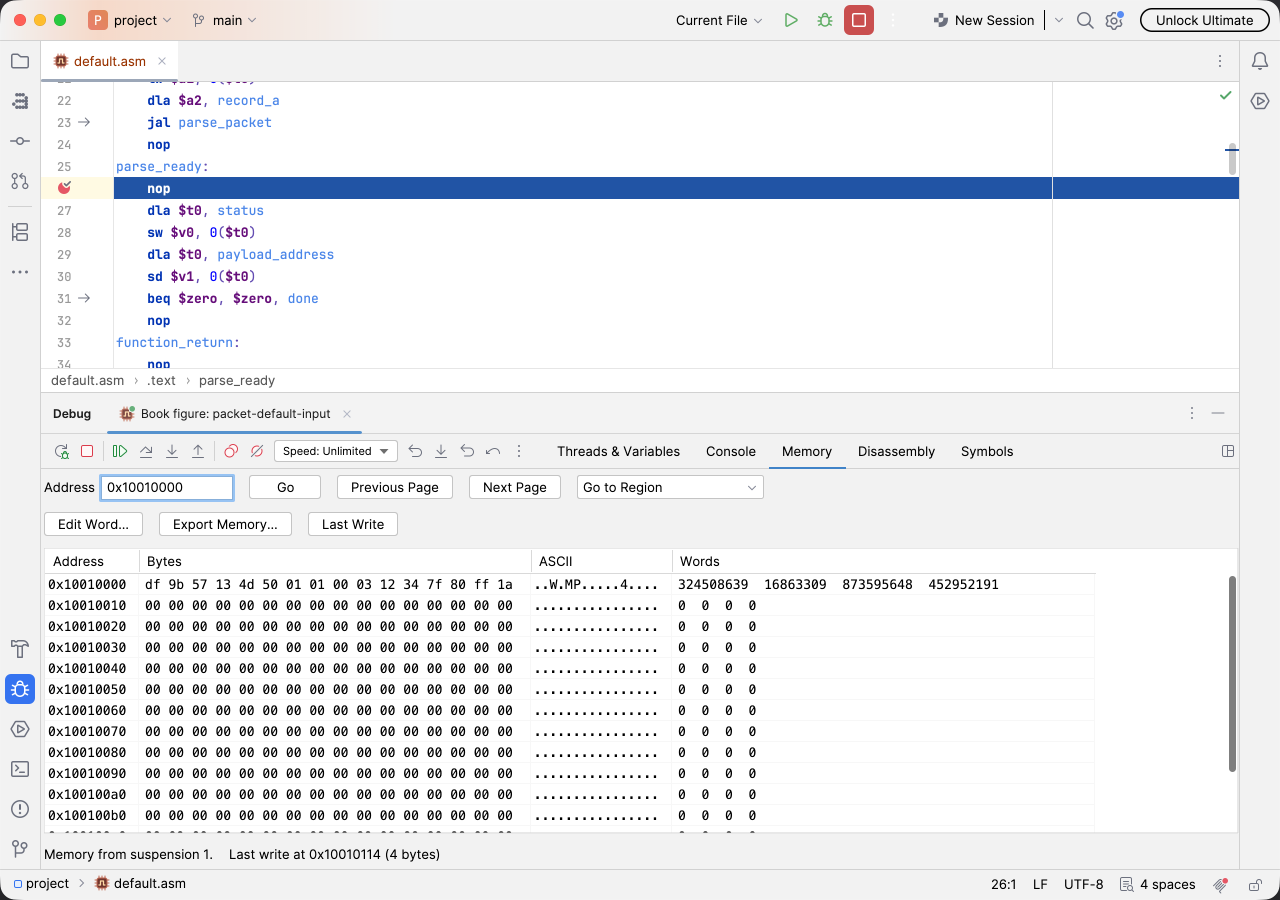
\includegraphics[artifact]{packages/013-binary-packet-parser/captures/f01-default/input.png}}
  \sbox6{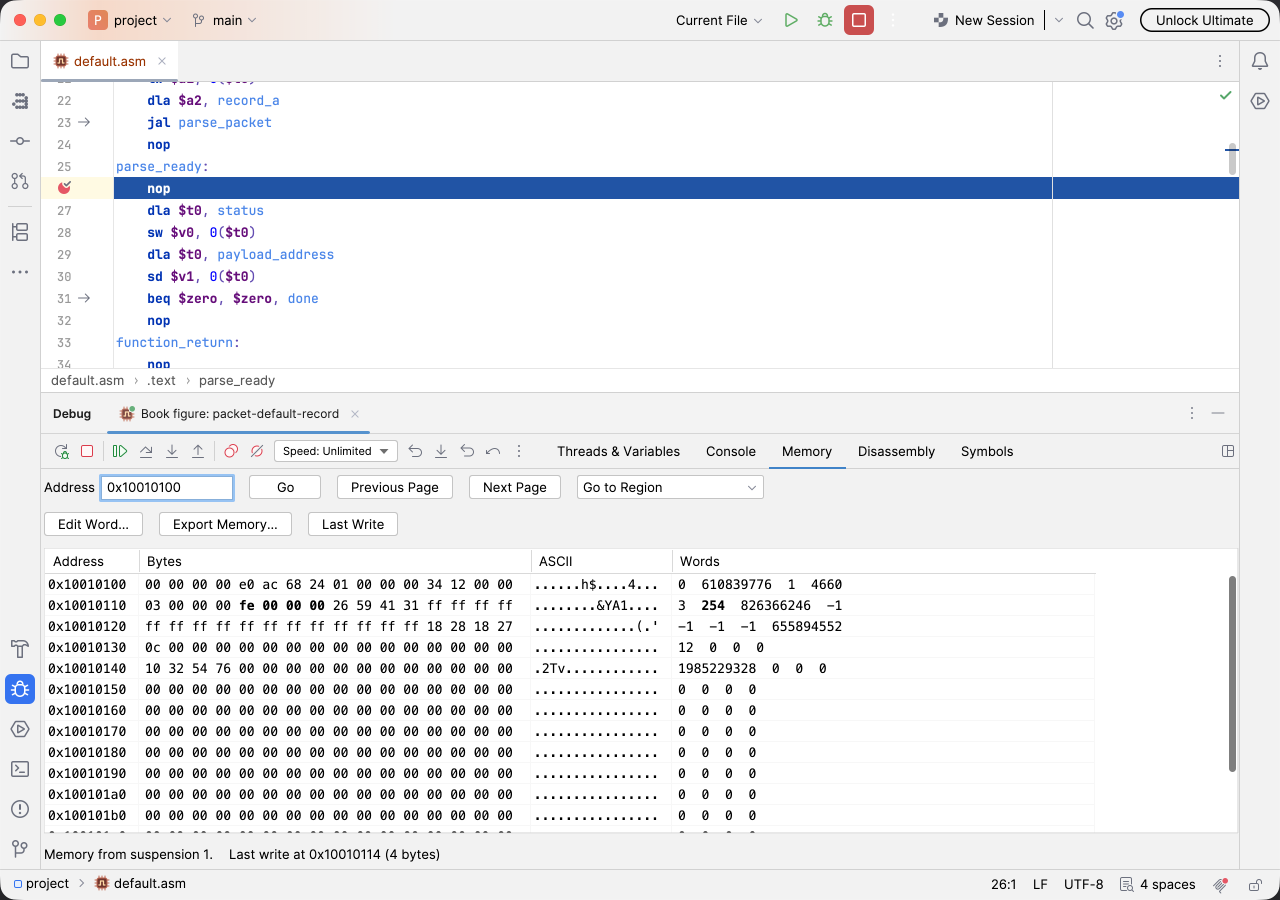
\includegraphics[artifact]{packages/013-binary-packet-parser/captures/f01-default/record.png}}
  \edef\MARSpacketdefaultsourceLeft{\the\dimexpr0.036718750\wd0\relax}
  \edef\MARSpacketdefaultsourceBottom{\the\dimexpr0.774444444\ht0\relax}
  \edef\MARSpacketdefaultsourceRight{\the\dimexpr0.713281250\wd0\relax}
  \edef\MARSpacketdefaultsourceTop{\the\dimexpr0.147777778\ht0\relax}
  \edef\MARSpacketdefaulthexLeft{\the\dimexpr0.246093750\wd0\relax}
  \edef\MARSpacketdefaulthexBottom{\the\dimexpr0.245555556\ht0\relax}
  \edef\MARSpacketdefaulthexRight{\the\dimexpr0.553906250\wd0\relax}
  \edef\MARSpacketdefaulthexTop{\the\dimexpr0.640000000\ht0\relax}
  \edef\MARSpacketdefaultdecimalLeft{\the\dimexpr0.246093750\wd2\relax}
  \edef\MARSpacketdefaultdecimalBottom{\the\dimexpr0.312222222\ht2\relax}
  \edef\MARSpacketdefaultdecimalRight{\the\dimexpr0.553906250\wd2\relax}
  \edef\MARSpacketdefaultdecimalTop{\the\dimexpr0.640000000\ht2\relax}
  \edef\MARSpacketdefaultinputLeft{\the\dimexpr0.034375000\wd4\relax}
  \edef\MARSpacketdefaultinputBottom{\the\dimexpr0.334444444\ht4\relax}
  \edef\MARSpacketdefaultinputRight{\the\dimexpr0.584375000\wd4\relax}
  \edef\MARSpacketdefaultinputTop{\the\dimexpr0.608888889\ht4\relax}
  \edef\MARSpacketdefaultrecordLeft{\the\dimexpr0.034375000\wd6\relax}
  \edef\MARSpacketdefaultrecordBottom{\the\dimexpr0.311111111\ht6\relax}
  \edef\MARSpacketdefaultrecordRight{\the\dimexpr0.584375000\wd6\relax}
  \edef\MARSpacketdefaultrecordTop{\the\dimexpr0.608888889\ht6\relax}
  \begin{tikzpicture}[alt={Five annotated details at parser return. Hexadecimal and native signed-decimal views show status twelve and payload address input plus eight. Input begins at 0x10010004 with the twelve valid packet bytes after its guard. Record A at 0x10010108 contains flags one, sequence 4660, payload length three and payload-sum residue 254. Caller status/pointer stores have not executed.}]
    \node[anchor=north west,inner sep=0,font=\small\bfseries] (source-title) at (6mm,0) {Next instruction after return};
    \node[anchor=north west,inner sep=0] (source) at ([yshift=-1mm]source-title.south west) {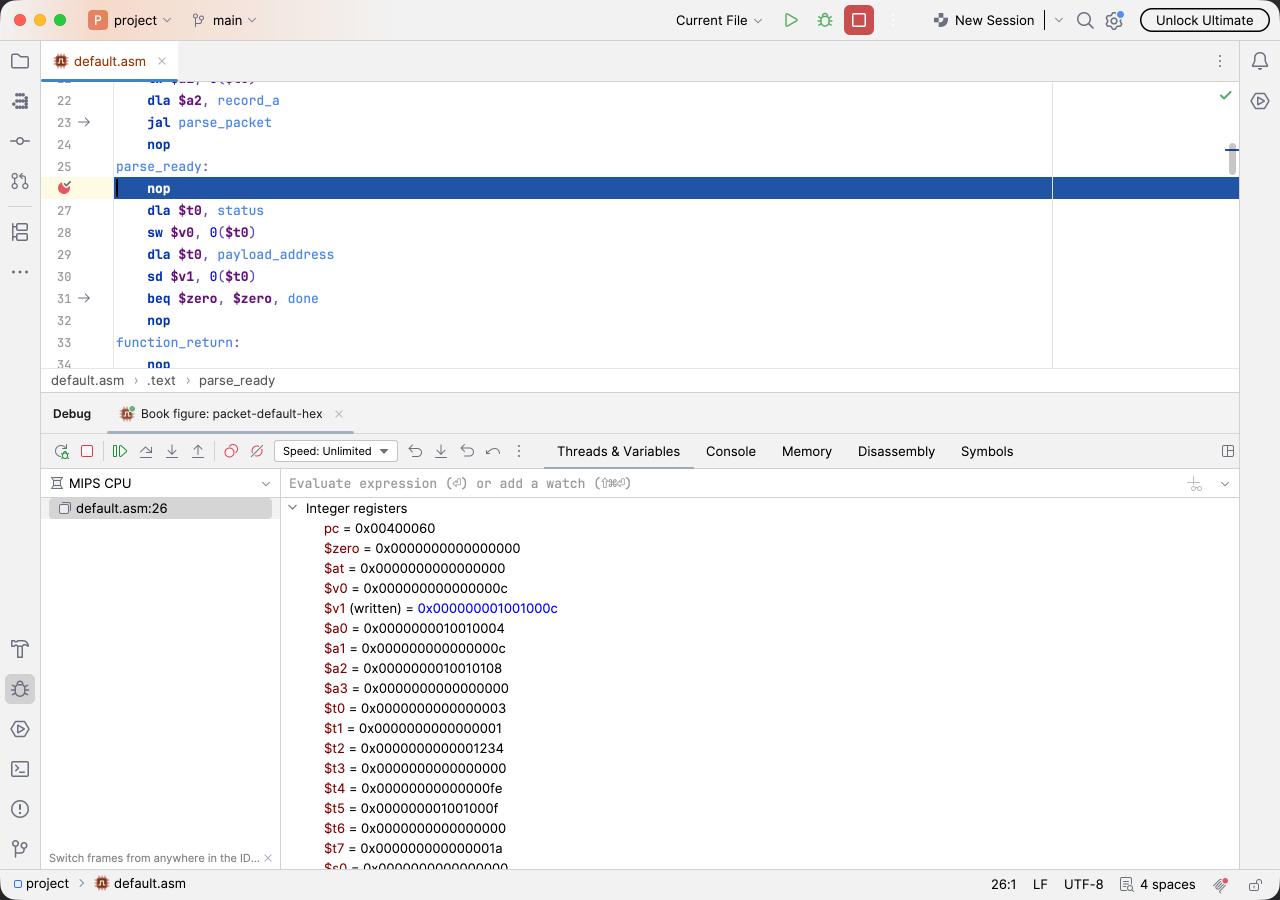
\includegraphics[width=0.54\linewidth,artifact,trim={\MARSpacketdefaultsourceLeft{} \MARSpacketdefaultsourceBottom{} \MARSpacketdefaultsourceRight{} \MARSpacketdefaultsourceTop{}},clip]{packages/013-binary-packet-parser/captures/f01-default/hex.png}};
    \begin{scope}[shift={(source.south west)},x={($(source.south east)-(source.south west)$)},y={($(source.north west)-(source.south west)$)}]
      \draw[black,line width=0.7pt] (0.215625000,0.057142857) rectangle (0.384375000,0.371428571);
      \node[draw=black,fill=white,circle,inner sep=1.5pt,font=\footnotesize] at ($(0.215625000,0.371428571)+(-3mm,0)$) {1};
    \end{scope}
    \node[anchor=north west,inner sep=0,font=\small\bfseries] (hex-title) at ([yshift=-3mm]source.south west) {Hexadecimal registers};
    \node[anchor=north west,inner sep=0] (hex) at ([yshift=-1mm]hex-title.south west) {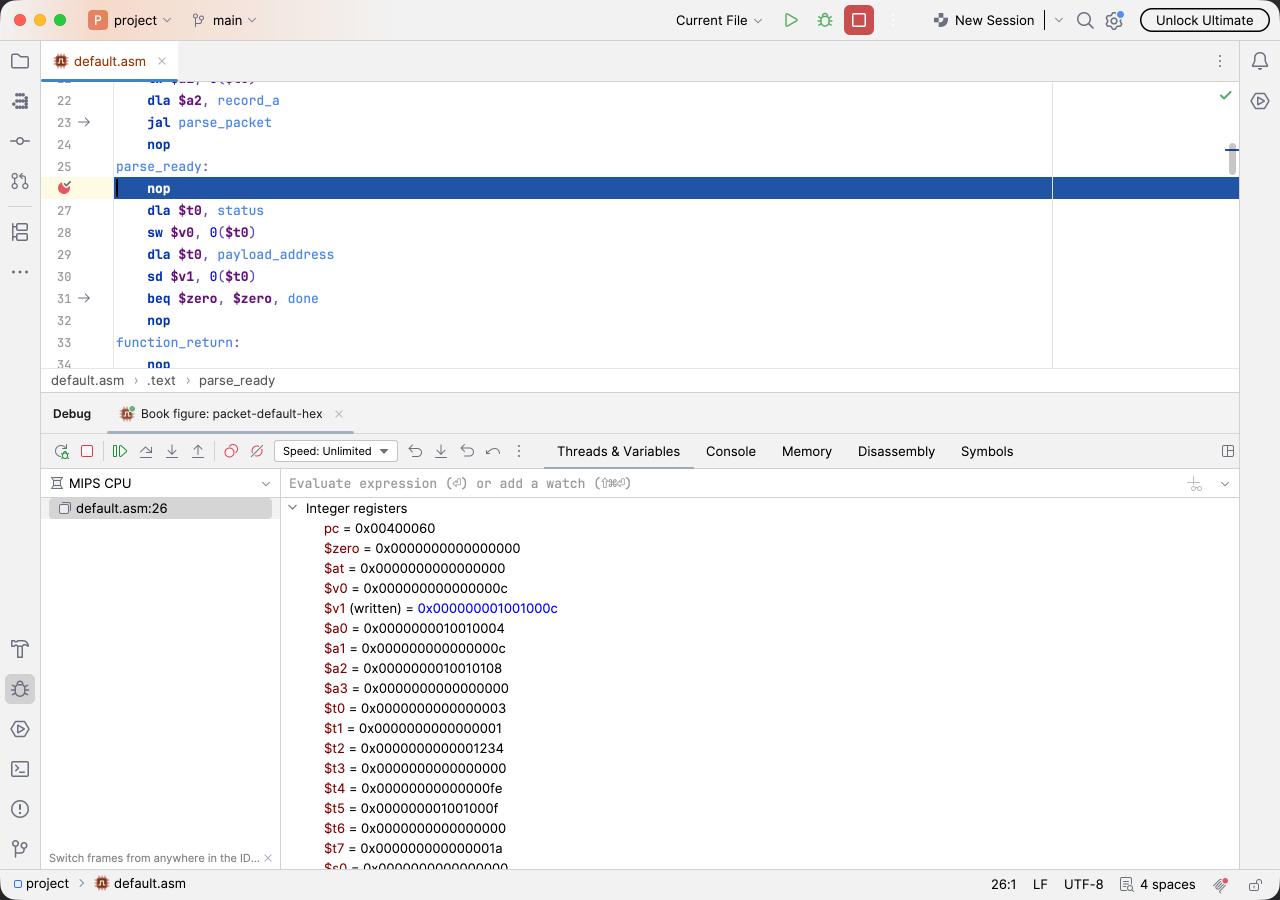
\includegraphics[width=0.42\linewidth,artifact,trim={\MARSpacketdefaulthexLeft{} \MARSpacketdefaulthexBottom{} \MARSpacketdefaulthexRight{} \MARSpacketdefaulthexTop{}},clip]{packages/013-binary-packet-parser/captures/f01-default/hex.png}};
    \begin{scope}[shift={(hex.south west)},x={($(hex.south east)-(hex.south west)$)},y={($(hex.north west)-(hex.south west)$)}]
      \draw[black,line width=0.7pt] (0.023437500,0.009708738) rectangle (0.953125000,0.980582524);
      \node[draw=black,fill=white,circle,inner sep=1.5pt,font=\footnotesize] at ($(0.023437500,0.980582524)+(-3mm,0)$) {2};
    \end{scope}
    \node[anchor=north west,inner sep=0,font=\small\bfseries] (decimal-title) at (0.58\linewidth,0 |- hex-title.north) {Signed return values};
    \node[anchor=north west,inner sep=0] (decimal) at ([yshift=-1mm]decimal-title.south west) {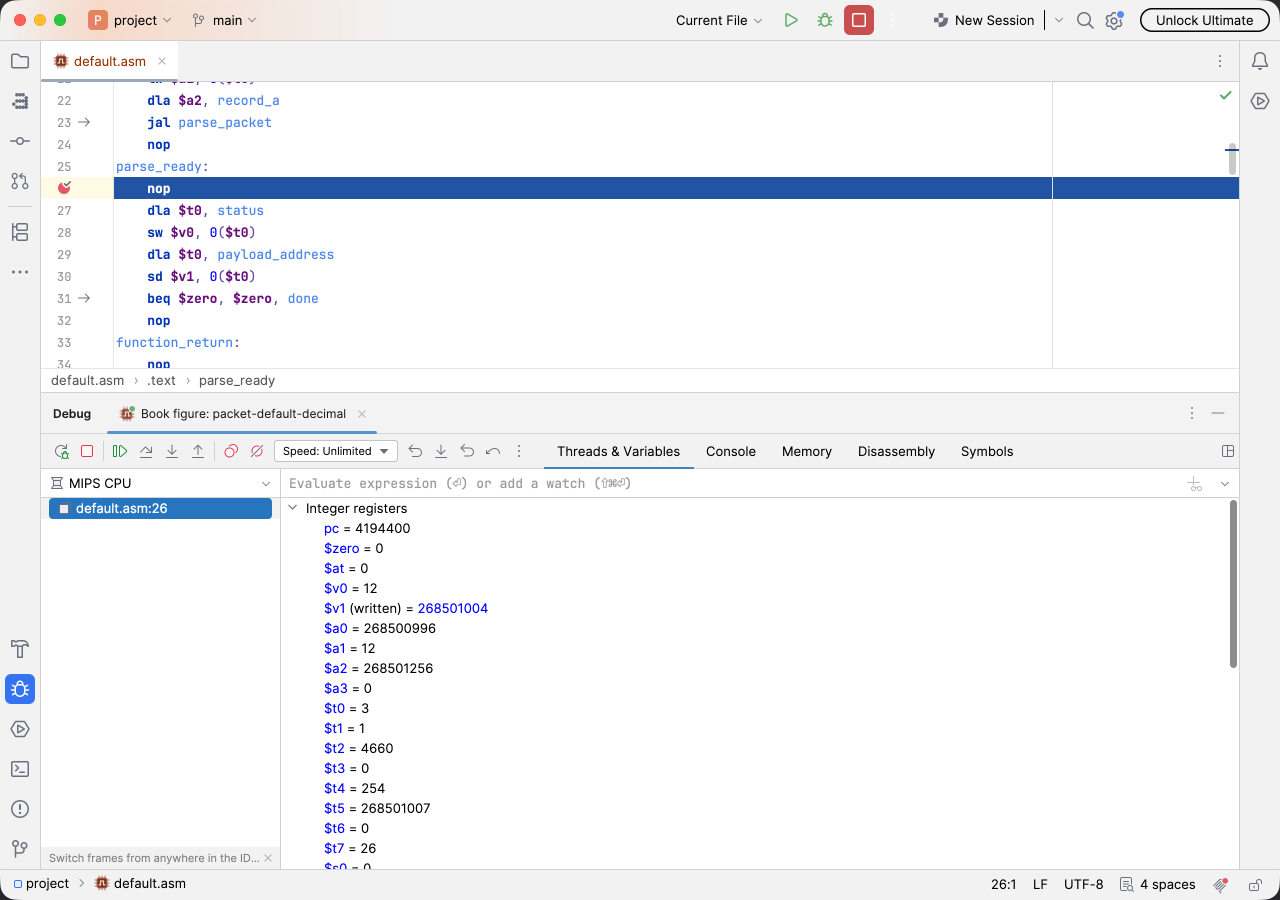
\includegraphics[width=0.42\linewidth,artifact,trim={\MARSpacketdefaultdecimalLeft{} \MARSpacketdefaultdecimalBottom{} \MARSpacketdefaultdecimalRight{} \MARSpacketdefaultdecimalTop{}},clip]{packages/013-binary-packet-parser/captures/f01-default/decimal.png}};
    \begin{scope}[shift={(decimal.south west)},x={($(decimal.south east)-(decimal.south west)$)},y={($(decimal.north west)-(decimal.south west)$)}]
      \draw[black,line width=0.7pt] (0.023437500,0.023255814) rectangle (0.683593750,0.953488372);
      \node[draw=black,fill=white,circle,inner sep=1.5pt,font=\footnotesize] at ($(0.023437500,0.953488372)+(-3mm,0)$) {3};
    \end{scope}
    \node[anchor=north west,inner sep=0,font=\small\bfseries] (input-title) at ([yshift=-3mm]hex.south west) {Mapped input bytes, including the preceding guard};
    \node[anchor=north west,inner sep=0] (input) at ([yshift=-1mm]input-title.south west) {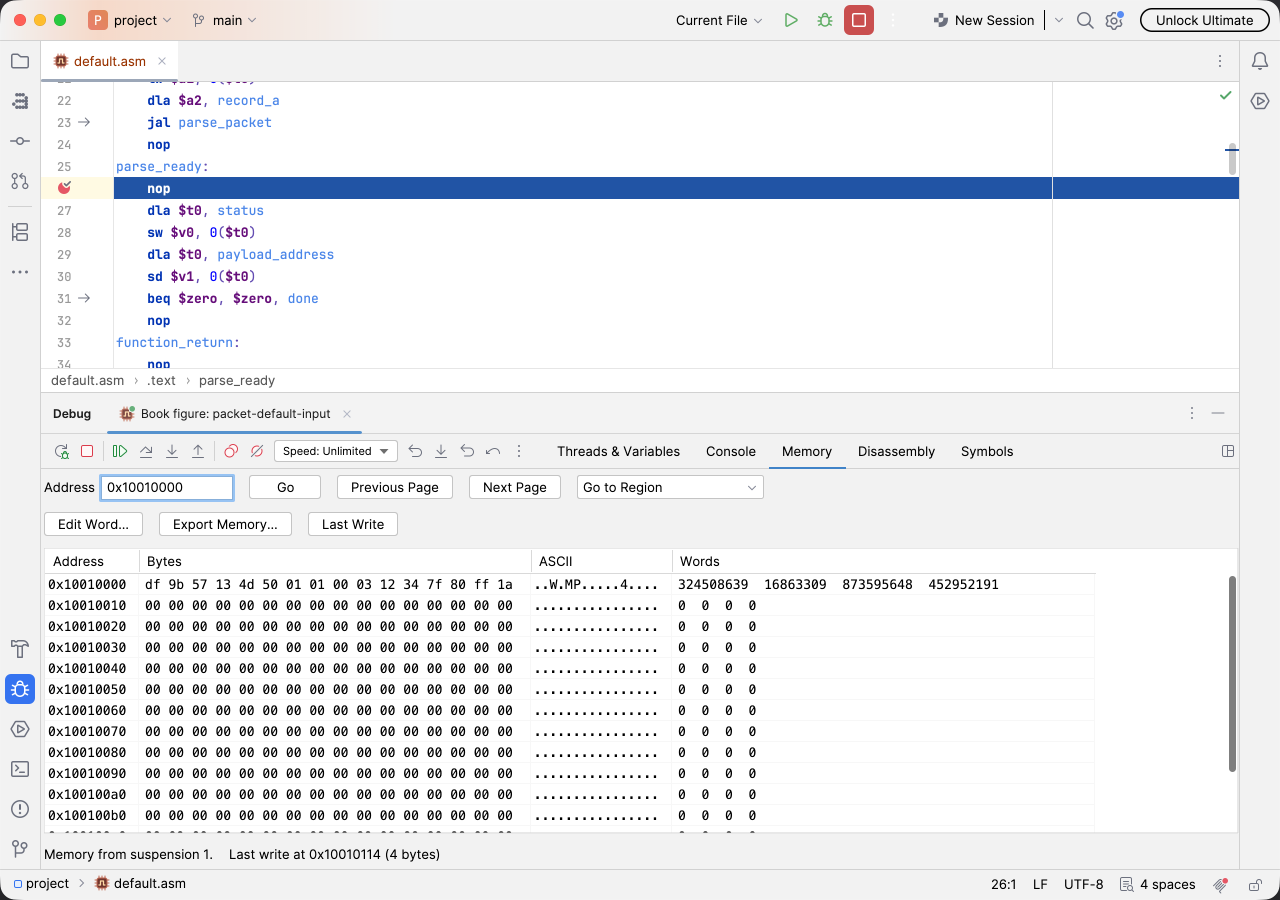
\includegraphics[width=0.84\linewidth,artifact,trim={\MARSpacketdefaultinputLeft{} \MARSpacketdefaultinputBottom{} \MARSpacketdefaultinputRight{} \MARSpacketdefaultinputTop{}},clip]{packages/013-binary-packet-parser/captures/f01-default/input.png}};
    \begin{scope}[shift={(input.south west)},x={($(input.south east)-(input.south west)$)},y={($(input.north west)-(input.south west)$)}]
      \draw[black,line width=0.7pt] (0.194672131,0.078431373) rectangle (0.997950820,0.490196078);
      \node[draw=black,fill=white,circle,inner sep=1.5pt,font=\footnotesize] at ($(0,0.490196078)+(-3mm,0)$) {4};
    \end{scope}
    \node[anchor=north west,inner sep=0,font=\small\bfseries] (record-title) at ([yshift=-3mm]input.south west) {Output record and its neighboring words};
    \node[anchor=north west,inner sep=0] (record) at ([yshift=-1mm]record-title.south west) {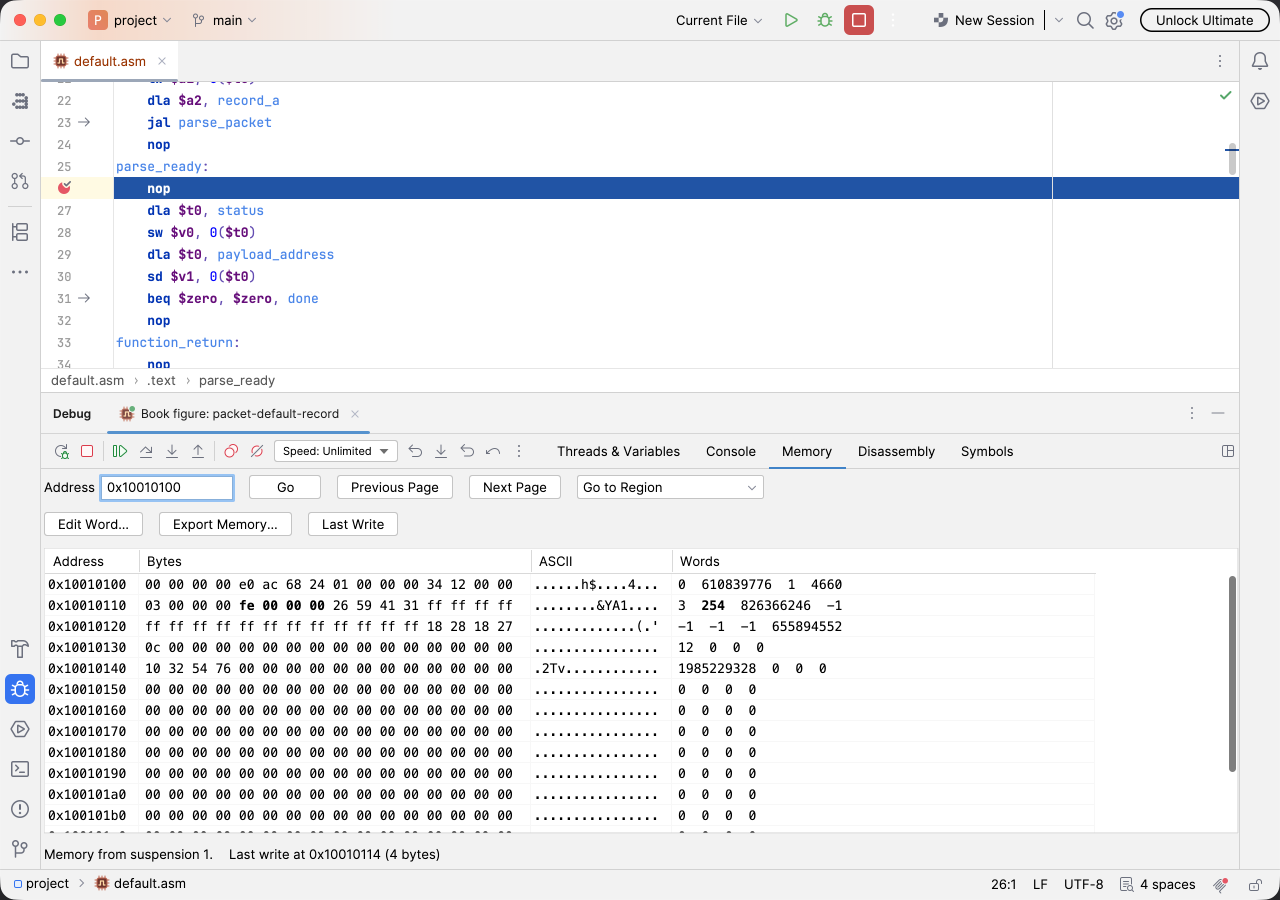
\includegraphics[width=0.84\linewidth,artifact,trim={\MARSpacketdefaultrecordLeft{} \MARSpacketdefaultrecordBottom{} \MARSpacketdefaultrecordRight{} \MARSpacketdefaultrecordTop{}},clip]{packages/013-binary-packet-parser/captures/f01-default/record.png}};
    \begin{scope}[shift={(record.south west)},x={($(record.south east)-(record.south west)$)},y={($(record.north west)-(record.south west)$)}]
      \draw[black,line width=0.7pt] (0.194672131,0.055555556) rectangle (0.997950820,0.638888889);
      \node[draw=black,fill=white,circle,inner sep=1.5pt,font=\footnotesize] at ($(0,0.638888889)+(-3mm,0)$) {5};
    \end{scope}
  \end{tikzpicture}
  \par\smallskip
  \begin{minipage}{\linewidth}
    \small
    \begin{enumerate}
      \setlength{\itemsep}{2pt}
            \setlength{\parsep}{0pt}
      \item The parser has returned to \texttt{parse\_ready}; the blue \texttt{nop} is next. The caller has not yet stored the status or payload address in its own data objects. Inspect return registers at this boundary, before exit later reuses \texttt{\$v0}.
      \item \texttt{\$a0 = 0x10010004} is the input pointer, \texttt{\$a1 = 0x0c} supplies twelve available bytes, and \texttt{\$a2 = 0x10010108} names the output. The returned \texttt{\$v1 = 0x1001000c} is input plus eight, the first payload byte. It aliases the input; no payload copy is made.
      \item The separate native decimal view shows \texttt{\$v0 = 12} and \texttt{\$v1 = 268501004}. The positive status counts this packet\textquotesingle s eight-byte header, three-byte payload and one-byte trailer. The two register views replay the same fixture and checkpoint with different display bases.
      \item The first four displayed bytes are the preceding guard. The packet starts at \texttt{4d 50} at \texttt{0x10010004}. Wire bytes \texttt{00 03} encode length 3; \texttt{12 34} encode sequence \texttt{0x1234}=4660, most significant byte first. Header sum 232, unsigned payload sum 510 and trailer 26 give $232+510+26=768$, a multiple of 256.
      \item The four record words occupy \texttt{0x10010108} through \texttt{0x10010117}: $[1,4660,3,254]$. The first two fields appear on the first debugger line and the other two on the next. Sequence bytes are now \texttt{34 12 00 00}, the simulator\textquotesingle s little-endian word representation. Residue 254 is $510\bmod256$. Neighboring padding, guards and record B are not fields of record A.
    \end{enumerate}
  \end{minipage}
  \caption{The default packet returns twelve consumed bytes, an aliased payload pointer and four decoded fields.}
  \label{capture:013-binary-packet-parser-f01-default}
  \label{packet-f01-default}
\end{figure}
\par
